\section{Estructura analítica}
    
Demostremos un lema técnico que nos ayudará a probar que las variedades afines (no singulares) admiten una estructura compleja.


\begin{lemma}\label{lemacubierta}
	Sea $M$ un espacio topológico Hausdorff y segundo numerable. Supongamos que existe una cubierta $\{W_\alpha\}_{\alpha\in I}$ de $M$ tal que cada $W_\alpha$ es una variedad compleja de dimensión $n$. Entonces $M$ es una variedad compleja de dimensión $n$.
\end{lemma}
\begin{proof}
	Sea 
	\begin{equation*}
		\mathcal{A}=\bigcup_{\alpha\in I}\mathrm{A}_\alpha
	\end{equation*}
	la unión de todos lo atlas de las variedades $W_\alpha$.
	Claramente los abiertos de $\mathcal{A}$ forman una cubierta para $M$, por lo que solo necesitamos probar que las cartas son compatibles para determinar que $M$ es una variedad compleja. Tomemos dos carta cualquiera
	\begin{equation*}
		    		(U,\varphi)\in\mathcal{A}_\alpha,\qquad (V,\psi)\in\mathcal{A}_\beta.
	\end{equation*}
	Consideremos la intersección $U\cap V$ y supongamos que $U\cap V\neq\emptyset$. Sea $x\in U\cap V$, entonces se tiene que
	\begin{equation*}
		x\in U\cap V\subset W_\alpha\cap W_\beta.
	\end{equation*}
	Observemos que $W_\alpha\cap W_\beta$ es un abierto en $W_\alpha$ (y en $W_\beta$), por lo que hereda la estructura de variedad compleja de $W_\alpha$ (respectivamente de $W_\beta$) al restringir su atlas.\\
	En particular, la carta $(U,\varphi)$, al ser carta de $W_\alpha$, cuando se restringe a $U\cap V$ sigue siendo un biholomorfismo desde $U\cap V$ (con la estructura de $W_\alpha$) hacía un abierto de $\cc^n$.\\
	Análogamente, la carta $ (V,\psi)$ restringida a $U\cap V$ es un biholomorfismo desde $U\cap V$ (con la estructura de $W_\beta$) hacía un abierto de $\cc^n$.\\
	De esta manera, ambas restricciones son carta holomorfas del mismo abierto $U\cap V$. Esto implica que las dos cartas pertenecen al atlas restringido de la variedad compleja $W_\alpha\cap W_\beta$. Más aún, la restricción de $(V,\psi)$ a $U\cap V$ es una aplicación holomorfa porque $(V,\psi)$ ya era holomorfa en $V$. Por lo tanto, la transición entre ellas
	\begin{equation*}
		  	\psi\circ\varphi^{-1}:\varphi(U\cap V)\longrightarrow \psi(U\cap V)
	\end{equation*} 
	es exactamente una función de transición entre dos cartas del mismo atlas sobre la variedad compleja $W_\alpha\cap W_\beta$. Como en ese atlas las transiciones son holomorfas, concluimos que $\psi\circ\varphi^{-1}$ es holomorfa en $\varphi(U\cap V)$. Esto prueba la compatibilidad de cualquier par de cartas de $\mathcal{A}$.
%	Sean $(U,\varphi)\in \mathcal{A}_\alpha$ y $(V,\psi)\in \mathcal{A}_\beta$ con $U\cap V\neq \emptyset$. Como $W_\alpha\cap W_\beta$ es un abierto tanto de $W_\alpha$ como de $W_\beta$, hereda ambas estructuras complejas. Así, las restricciones de $(U,\varphi)$ y $(V,\psi)$ a $U\cap V$ son cartas holomorfas de $W_\alpha\cap W_\beta$. Con lo cual, la función de transición
%	\begin{equation*}
%		\psi\circ\varphi^{-1}
%	\end{equation*} 
%	es holomorfa. Esto prueba la compatibilidad de todas las cartas de $\mathcal{A}$.
\end{proof}

\begin{theorem}\parencite[Teo. 3.37]{carlosga}\label{teocarlos}
	Sea $V\subset\cc^n$ una variedad algebraica afín de dimensión $r$. Si $p\in V$ es un punto no singular, entonces existe una vecindad $U\subset \cc^n$ de $p$ y $f_1,\dots,f_{n-r}\in\cc[z_1,\dots,z_n]$ polinomios tales que 
	\begin{equation*}
		V\cap U=\{q\in U:f_1(q)=\cdots=f_{n-r}(q)=0\}.
	\end{equation*}
\end{theorem}

Este teorema nos dice que aunque nuestra variedad algebraica no sea globalmente de intersección completa, localmente sí debe estar definida por $n-r$ ecuaciones. Por teorema de la función implícita, veremos que $V$ localmente es una variedad compleja de dimensión $r$.

\begin{example}
	Considemos la curva monomial
	\begin{align*}
		\Phi:\cc\longrightarrow \cc^3\\
		t\mapsto (t^3,t^4,t^5).
	\end{align*}
	Su imagen es la curva (véase figura \ref{fig:curva-monomial})
	\begin{equation*}
		C=\{(t^3,t^4,t^5)\in\cc^3: t\in\cc\}.
	\end{equation*}
	cuyo ideal asociado está generado por
	\begin{equation*}
		I(C)=\langle y^2-xz,x^3-yz,z^2-x^2y \rangle\subset \cc[x,y,z].
	\end{equation*}
	Esto implica que el ideal de $C$ requiere tres generadores, y en particular, $C$ no es de intersección completa. Sin embargo, al ser una curva intuitivamente debería estar generada por solo dos ecuaciones.
	
	Sea $p=(1,1,1)\in C$ y consideremos la vecindad afín
	\begin{equation*}
		U=\{(x,y,z)\in\cc^3:x\neq 0\}=Z(x)^c.
	\end{equation*}
	Supongamos que 
	\begin{equation*}
		y^2-xz=0,\qquad\text{y}\qquad yz-x^3=0.
	\end{equation*}
	entonces
	\begin{equation*}
		x(z^2-x^2y)=xz^2-x^3y=y(yz-x^3)-z(y^2-xz)=0.
	\end{equation*}
	Como $x\neq 0$ en $U$, entonces
	\begin{equation*}
		z^2-x^2y=0.
	\end{equation*}
	Esto significa que en $U$, la condición anterior se reduce de las otras dos. Por lo tanto,
	\begin{equation*}
		U\cap C=Z(y^2-xz,yz-x^3).
	\end{equation*}
	\begin{center}
		\begin{figure}[H]
			\centering
			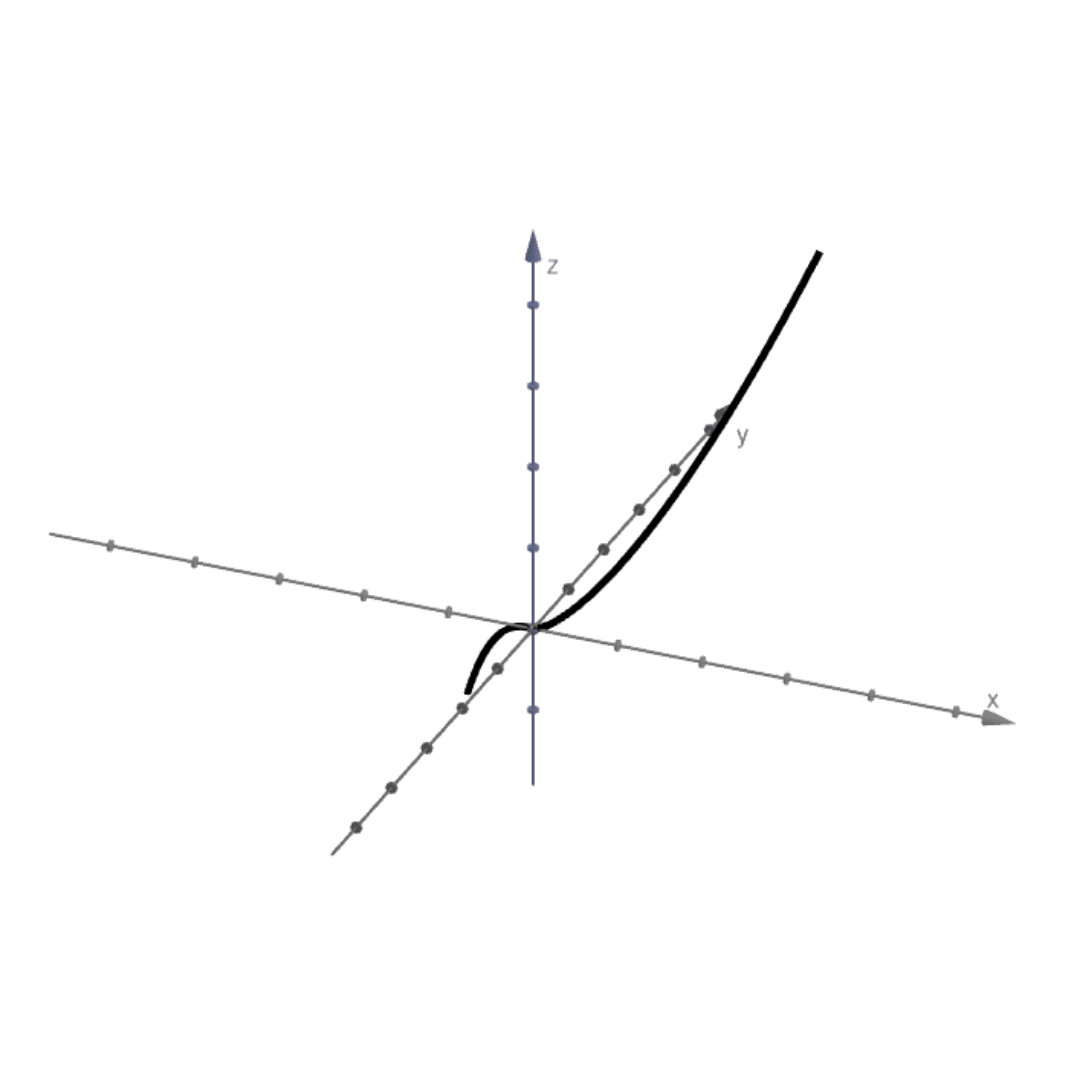
\includegraphics[width=0.3\linewidth]{Imagenes/Curva monomial}
			\caption{Curva monomial $Z(y^2-xz,yz-x^3,z^2-x^2y)$.}
			\label{fig:curva-monomial}
		\end{figure}
	\end{center}
\end{example}

\begin{corollary}\label{analiticoafin}
	Sea $V\subset \cc^n$ una variedad afín no singular de dimensión $r$. Entonces $V$ es una variedad compleja de dimensíon $r$.
\end{corollary}
\begin{proof}
	Sea $p\in V$ un punto albitrario. Como $V$ es no singular de dimensión $r$, por el teorema \ref{teocarlos}, existe una vecindad $U_p\subset V$ de $p$ y polinomios 
	\begin{equation*}
		h_1,\dots,h_{n-r}\in\cc[z_1,\dots,z_n]
	\end{equation*}
	tales que
	\begin{equation*}
		V\cap U_p=\{q\in U_p:h_1(q)=\cdots=h_{n-r}(q)=0\},
	\end{equation*}
	y la matriz jacobiana $(\frac{\partial h_i}{\partial z_j}(p))$ tiene rango $n-r$.\\
	De esto, $0\in \cc^{n-r}$ es un valor regular de la aplicación holomorfa $h=(h_1,\dots,h_{n-r}):U_p\subset\cc^n\to\cc^{n-r}$. Por el ejemplo \ref{interseccioncompleja}, $V\cap U_p$ es una variedad compleja de dimensión
	\begin{equation*}
		n-(n-r)=r.
	\end{equation*}
	Como $p$ fue cualquier punto, obtenemos una cubierta para $V$
	\begin{equation*}
		V=\bigcup_{p\in V}U_p.
	\end{equation*} 
	donde cada $U_p$ es una variedad compleja de dimensión $r$. Finalmente, aplicando el lema \ref{lemacubierta}, $V$ es una variedad compleja de dimensión $r$.
\end{proof}

Dado que toda variedad algebraica afín admite una estructura de variedad compleja, vale la pena preguntarnos si el recíproco es verdad. Es decir, toda variedad compleja se puede realizarse como una variedad algebraica afín. La respuesta a esta cuestión es negativa, pues en primer lugar, las variedades algebraicas afines son conjuntos cerrados de $\cc^n$. De hecho, incluso entre las variedades complejas cerradas en $\cc^n$ existen ejemplos no algebraicas. Esto significa que existen muchas más variedades complejas que variedades algebraicas, por lo que motiva el problema de determinar bajo qué condiciones una variedad compleja admite una realización algebraica.

\begin{example}[Superficie de Riemann no algebraica]\label{graficadelseno}
	Sea
	\begin{equation*}
		X=\{(z,w)\in\mathbb \cc^2:\ w=\sin z\}
	\end{equation*}
	la gráfica de $\sin z$. Entonces $X$ es una superficie de Riemann (de hecho biholomorfa a $\cc$ mediante la proyección $\pi(z,\sin z)=z$) y no es compacta. Supongamos que existe un polinomio no cero $P(z,w)\in\cc[z,w]$ tal que
	\begin{equation*}
		P(z,\sin z)= 0\qquad\text{para todo }z\in\cc.
	\end{equation*}
	Escribamos
	\begin{equation*}
		P(z,w)=\sum_{j=0}^m a_j(z)w^j,\qquad a_j(z)\in\mathbb \cc[z].
	\end{equation*}
	Al evaluar en $w=0$ obtenemos el polinomio $a_0(z)=P(z,0) $. Como $P(z,\sin z)=0$, entonces para todo $z$ tal que $\sin z=0$ (es decir $z=n\pi,\ n\in\mathbb{Z}$) se cumple que $P(z,0)=0$. Así $a_0(z)$ tiene infinitos ceros y por ser un polinomio en $\cc[z]$ debe ser idénticamente cero.
	
	Con lo cual, $w$ divide a $P(z,w)$ en $\cc[z,w]$, es decir existe $P_1\in\cc[z,w] $ tal que
	\begin{equation*}
		P(z,w)=wP_1(z,w)
	\end{equation*}
	Con esto tenemos que
	\begin{equation*}
		0=P(z,\sin z)=\sin zP_1(z,\sin z),
	\end{equation*}
	y como $\sin z$ no es la función cero, entonces $ P_1(z,\sin z)=0$. Usando el mismo razonamiento, obtenemos que $P$ es divisible por $w^k$ para todo $k\geq 1$. Esto sólo es posible si $P$ es el polinomio cero, contradiciendo la hipótesis de que $P\neq0$. Por tanto, $X$ no es algebraica. 
	\begin{figure}[H]
		\centering
		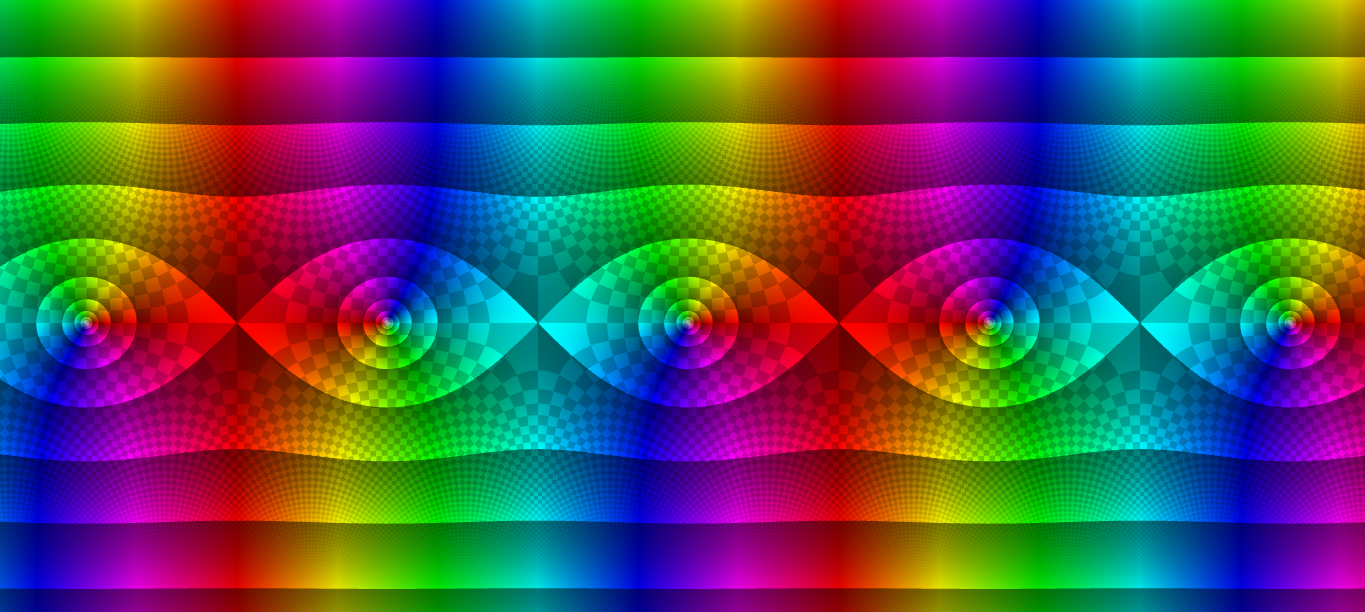
\includegraphics[width=0.5\linewidth]{Imagenes/Grafica del seno}
		\caption{Gráfica de la función seno}
		%			\caption{La función seno tiene una cantidad infinita de ceros la recta $w=0$. Por lo tanto, si la gráfica del seno fuera algebraica, al intersectar con la recta $w=0$ debería ser algebraica, lo cual no es posible.}
		\label{fig:grafica-del-seno}
	\end{figure}
\end{example}


\begin{definition}
	Sea $V\subset\pp^n$ una variedad algebraica y consideremos $V=\bigcup_{i=0}^n V_i$ la cubierta estandar afín. Definimos la \textbf{dimensión} de $V$ como el máximo de las dimensiones de las variedades afines $V_i\subset\cc^n$.
\end{definition}

En particular, la dimensión es una propiedad local e intrinseca de la variedad  algebraica, sin importar el espacio ambierte donde se encuentre.

\begin{remark}\label{dimcubierta}
	Denotemos por $\cc(V)$ al campo de funciones racionales de la variedad algebraica (afín o proyectiva) $V$. De geometría algebraica (por ejemplo véase \parencite[Cap. 1 Sec. 3]{Harts}) sabemos que si $V$ es afín, entonces
	\begin{equation*}
		\trdeg_{\cc} \cc(V)=\dim V.
	\end{equation*}
	Además, si $V\subset \pp^n$ es una variedad algebraica que no está totalmente contenida en $Z(z_i)$, entonces 
	\begin{equation*}
		\cc(V)\cong \cc(V_i),\qquad \text{con }V_i\text{ como variedad afín}.
	\end{equation*}
	De esta manera, si $V\subset\pp^n$ es una variedad algebraica, entonces para cada $i=0,1,\dots, n$ 
	\begin{equation*}
		\cc(V)\cong \cc(V_i)
	\end{equation*}
	si $V$ no está totalmente contenida en $Z(z_i)$. Asi,
	\begin{equation*}
		\trdeg_{\cc}\cc(V)=\trdeg_{\cc}\cc(V_i)=\dim V_i.
	\end{equation*}
	Por lo tanto, la dimensión de todas las variedades afines $V_i$ es igual a la dimensión de la variedad $V$.
\end{remark}

\begin{definition}
	Sea $V\subset\pp^n$ una variedad algebraica de dimensión $d$ y tomemos su cubierta afín
	\begin{equation*}
		V=\bigcup_{i=0}^n V_i
	\end{equation*}
	Decimos que la variedad $V$ es \textbf{no singular} si todos sus puntos son no singulares en todas las variedades afines. Es decir, las variedades afines $V_i$ son no singulares.
\end{definition}

Por definición, si $V\subset\pp^n$ es no singular, entonces $V$ está cubierta por $n+1$ variedades complejas (especificamente, está cubierto por abiertos en $V$ homeomorfos a una variedad compleja). Aprovecharemos esto para probar que $V$ también es una variedad compleja, pero determinemos antes las propiedades topológicas básicas de las variedades algebraicas.

\begin{lemma}\label{topovariedades}
	Toda variedad algebraica proyectiva es Hausdorff, segundo numerable y compacto (respecto a la topología compleja).
\end{lemma}

\begin{proof}
	Sea $X\subset \pp^n$ una variedad algebraica proyectiva. Notemos que $X$ como subespacio de $\pp^n$ es Hausdorff y segundo numerable. Solo es necesario demostrar que es compacto. Consideremos $X_i=X\cap U_i$ la cubierta afín de $X$. Lo que haremos es demostrar que cada $X_i$ es cerrado. Así, $X$ será cerrado por ser unión finita de cerrados y como $\pp^n$ es compacto, entonces $X$ es compacto.\\
	Como $X$ es variedad algebraica proyectiva, existen $F_k\in\cc[x_0,x_1,\dots,x_n]$ polinomios homogéneos tal que
	\begin{equation*}
		X=Z(F_1,F_2,\dots, F_k)        
	\end{equation*}
	Haremos la prueba para $i=0$, pero es análogo para todo $i=1,\dots, n$.
	Notemos que
	\begin{align*}
		\phi_0(X_0)=Z(f_1,f_2,\dots, f_n)
	\end{align*}
	donde 
	\begin{equation*}
		f_j(x_1,\dots,x_n)=F_j\left(1,x_1,\dots,x_n\right)
	\end{equation*}
	para cada $j=1,2\dots,k$. Esto porque
	\begin{align*}
		\phi_0(X_i)&=\{\phi([1:x_1:\dots:x_n]):[1:x_1.\dots:x_n]\in X_i\}\\
		&=\{(x_1,x_2,\dots,x_n):[1:x_1:\dots:x_n]\in X_i\}\\
		&=\{(x_1,x_2,\dots,x_n):F_j[1:x_1:\dots:x_n]=0, \text{ para toda } j=1,2\dots k\}\\
		&=\{(x_1,x_2,\dots,x_n):f_j(x_1,\dots,x_n)=0, \text{ para toda } j=1,2\dots k\}\\
		&=Z(f_1,f_2,\dots,f_j)\subset \cc^n
	\end{align*}
	Así
	\begin{equation*}
		\phi_0(X_0)=Z(f_1,f_2,\dots,f_j)=\bigcap_{k=1}^jZ(f_k)=\bigcap_{k=1}^jf_k^{-1}(0)
	\end{equation*}
	Por lo tanto, $\phi_0(X_0)$ es cerrado por ser intersección de cerrados y como $\phi$ es un homeomorfismo, entonces $X_0$ es cerrado.
\end{proof}

La conexidad de las variedades algebraicas es un hecho para nada trivial, pero es una propiedad muy importante que necesitamos considerar. Una prueba de esta propiedad se puede consultar en \parencite[Cap. 4 Sec. 4.2]{carlosga} o en \parencite[Cap. VII Sec. 2]{shafarevich2016basic}. Más aún, también podemos verlo como un caso particular del teorema \ref{irreducibleconexo}. Por lo tanto, podemos concluir que:

\begin{theorem}\label{varalg}
	Sea $V\subset\pp^n$ una variedad algebraica no singular de dimensión $r$. Entonces $V$ es una variedad compleja conexa compacta de dimensión $r$.    	
\end{theorem}
\begin{proof}
	Sea $V\subset\pp^n$ una variedad algebraica no singular de dimensión $r$ y consideremos su cubierta estándar 
	\begin{equation*}
		V=\bigcup_{i=0}^n V_i.
	\end{equation*}
	Supongamos que $V\not\subset Z(z_i)$ para todo $i=0,1,\dots,n$. Por la observación \ref{dimcubierta}, las variedades afines $V_i$ dimensión $r$. Luego, por definición de no singular, las $V_i$ son no singulares. De esta manera, por el corolario \ref{analiticoafin}, las variedades afines $V_i$ tienen estructura de variedad compleja de dimensión $r$.\\
	Por el lema \ref{lemacubierta}, como $V$ está cubierto por las variedades complejas $V_i$, concluimos que $V$ tiene estructura de variedad compleja de dimensión $r$.\\
	Ahora, si $V$ está totalmente contenida en algún $Z(z_i)$, digamos $i=0$, entonces $V_i=\emptyset$. Por lo que
	\begin{equation*}
		V=\bigcup_{i=0}^n V_i=\bigcup_{i=1}^n V_i
	\end{equation*}
	y la demostración sigue siendo válida.
	
	Por el lema \ref{topovariedades}, $V$ es compacta. Además, la conexidad de $V$ se sigue de la irreducibilidad de las variedades algebraicas proyectivas (véase la discusión previa al teorema). Por lo tanto, $V$ es una variedad compleja conexa y compacta de dimensión r.
\end{proof}